
\section{Parte 2: Análisis dinámico del pozo finito asimétrico [50 puntos]}
 
Consideremos ahora el pozo finito asimétrico definido por el potencial
\begin{equation}
U(x) = \begin{cases} U_1, & x < 0, \\ 0, & 0 \leq x < L, \\ U_2, & x \geq L, \end{cases} \qquad \{U_1, U_2\} > 0, \qquad U_2 \geq U_1, \qquad c \equiv \frac{U_2}{U_1} \geq 1, \tag{10}
\end{equation}

\begin{figure}
    \centering
    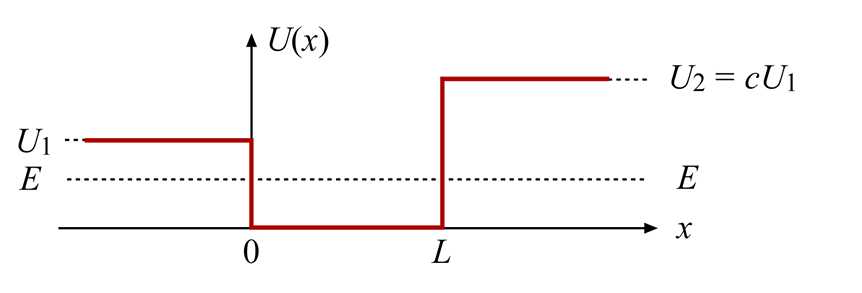
\includegraphics[width=0.5\linewidth]{figures/p2_asymmetric_well_assignment.png}
    \caption{Pozo infinito de potencial de anchura $L$ y paredes con potenciales diferentes}
    \label{fig:1}
\end{figure}
que se muestra en la Fig. 1. Sin perder generalidad, asumimos que $U_2 \geq U_1$, por lo que el factor de proporcionalidad $c \geq 1$. El factor $c$ se considera como un parámetro de asimetría entre ambas paredes. Observen que el pozo está definido entre $x = 0$ y $x = L$, pues al no ser simétrico, ya no tiene ninguna ventaja definirlo simétricamente alrededor de $x = 0$. Definimos el inicio del pozo en $x = 0$ para facilitar evaluaciones en esa frontera.
 
\begin{pregunta}{1.}
Escribe la forma general de las eigenfunciones $\varphi_n(x)$ del pozo asimétrico. Nota que el pozo tiene tres secciones de potencial constante. Asume que la energía de la partícula está en el rango $0 < E < U_1$. Observa que el pozo no tiene simetría, por lo que los estados $\varphi_n(x)$ no tienen paridad, como sí existía en el potencial simétrico. Esto último va a tener un impacto en la forma en la que escribas la forma del estado en la zona central de atrapamiento.
\end{pregunta}


% Figura del pozo (dibujo a mano): U_1 para x<0, 0 en 0<=x<L, U_2 para x>=L, nivel E por debajo de U_1
\begin{equation*}
U_2 = cU_1, \qquad c = \frac{U_2}{U_1} \geq 1, \qquad 0 \leq E \leq U_1 \leq U_2
\end{equation*}

Se observa que son tres áreas con potencial finito... La onda debe cumplir la ec. de Schrödinger $\forall x$
\begin{equation*}
-\frac{\hbar^2}{2m}\partial^2_x\varphi_ + V\varphi = E\varphi
\end{equation*}

Para $0<x<L$: $E - V = E$, dado que $V=0$.
\begin{equation*}
\Rightarrow -\frac{\hbar^2\partial^2\varphi}{2m} = E\varphi \Rightarrow \varphi = A\cos(\omega x) + B\sin(\omega x) \quad \text{donde} \quad \omega \equiv \sqrt{\frac{2mE}{\hbar^2}}
\end{equation*}

Para $x<0$: Si $U_1 - E > 0$
\begin{equation*}
\Rightarrow \partial^2\varphi = \frac{2m}{\hbar^2}(-E+U_1)\varphi = \kappa^2\varphi, \qquad \kappa \equiv \sqrt{\frac{2m(U_1-E)}{\hbar^2}}, \qquad \kappa > 0 \ldots
\end{equation*}
\begin{equation*}
\Rightarrow \varphi = C_1 e^{\kappa x} + C_2 e^{-\kappa x}
\end{equation*}
Claramente, el segundo término no es normalizable para $x<0$, por lo que $C_2 = 0$. Sea $C_1 = C$
\begin{equation*}
\Rightarrow \varphi(x) = C e^{+\kappa x}
\end{equation*}

Para $x>L$: $U_2 - E > 0$. Similar al pasado sea
\begin{equation*}
\gamma \equiv \sqrt{\frac{2m(U_2-E)}{\hbar^2}} = \sqrt{\frac{2m(cU_1-E)}{\hbar^2}}
\end{equation*}
\begin{equation*}
\Rightarrow \varphi = De^{-\gamma x}
\end{equation*}

Ahora, juntamos las soluciones para formar una solución continua.
\begin{equation}
\varphi(x) = \begin{cases} C e^{+\kappa x}, & x<0, \\ A\cos(\omega x) + B\sin(\omega x), & 0 \leq x < L, \\ De^{-\gamma x}, & x \geq L. \end{cases}
\label{eq: phi cases asim}
\end{equation}

Como el potencial no es simétrico, los estados $\varphi_n(x)$ no tienen paridad definida, por lo que en la zona central se conservan ambos términos, $\cos(\omega x)$ y $\sin(\omega x)$, con $A$ y $B$ en general distintos de cero. Las constantes $\omega$, $\kappa$ y $\gamma$ dependen de $E_n$.


 
\begin{pregunta}{2.}
Encuentra la ecuación característica para las eigenenergías $E_n$ de los estados estacionarios $\varphi_n(x)$ de una partícula atrapada en el potencial de pozo asimétrico. \textit{Hint: Puedes intentar la estrategia del problema 4 de la parte 1 del pozo simétrico. Opcionalmente, puedes parametrizar como lo hicimos en clase para que la ecuación quede más compacta y dependa solo de un parámetro.}
\end{pregunta}



Ahora las constantes $A,B,C,D$ de $\varphi(x)$ en la ecuación \ref{eq: phi cases asim} se calculan. Estas soluciones y sus derivadas deben coincidir en las condiciones de frontera \dots

\noindent En $x=0$:
\begin{equation*}
\boxed{C = A}, \qquad C\kappa = B\omega, \qquad \boxed{B = +\frac{\kappa}{\omega}C}
\end{equation*}

\noindent En $x=L$:
\begin{align*}
A\cos(\omega L) + B\sin(\omega L) &= De^{-\gamma L} \\
-A\omega\sin(\omega L) + B\omega\cos(\omega L) &= -D\gamma e^{-\gamma L}
\end{align*}

Remplazando a $A$ y $B$ en términos de $C$ \dots

\begin{align}
C\cos(\omega L) + \frac{\kappa}{\omega}C\sin(\omega L) &= De^{-\gamma L} \label{C1} \\
-C\omega\sin(\omega L) + \kappa C\cos(\omega L) &= -D\gamma e^{-\gamma L} \label{C2}
\end{align}

Multiplicando por $\kappa$ \ref{C1} y luego restando a \ref{C2}
\begin{equation*}
\frac{\kappa^2}{\omega}C\sin(\omega L) + C\omega\sin(\omega L) = D[\kappa+\gamma]e^{-\gamma L}
\end{equation*}
\begin{equation*}
C\sin(\omega L)\left[\frac{\kappa^2}{\omega} + \omega\right] = De^{-\gamma L}[\kappa+\gamma]
\end{equation*}
\begin{equation*}
\boxed{D = C e^{\gamma L} \left[\frac{\sin(\omega L)\left[\kappa^2 + \omega^2\right]}{\omega[\gamma+\kappa]}\right]}
\end{equation*}

Ahora, ya tenemos todas las constantes en términos de $C$. Sin embargo de las ecuaciones \ref{C1}, \ref{C2}, podemos también obtener una ecuación que relacione las variables $\omega, \gamma, \kappa$, lo que nos permitiría obtener los estados de energía permisibles.

Multiplicando \ref{C1} por $\gamma$ y despejando $\frac{D}{C}e^{-\gamma L}\gamma$
\begin{equation*}
\frac{D}{C}\gamma e^{-\gamma L} = \gamma\cos(\omega L) + \frac{\kappa}{\omega}\gamma\sin(\omega L) = -\kappa\cos(\omega L) + \omega\sin(\omega L)
\end{equation*}
\begin{equation*}
\Rightarrow \gamma\cos(\omega L) + \frac{\kappa}{\omega}\gamma\sin(\omega L) = -\kappa\cos(\omega L) + \omega\sin(\omega L)
\end{equation*}
\begin{equation*}
\cos(\omega L)\left[\gamma + \kappa\right] = \sin(\omega L)\left[\omega - \frac{\kappa\gamma}{\omega}\right]
\end{equation*}
\begin{equation*}
\Rightarrow \tan(\omega L) = \frac{\gamma + \kappa}{\omega - \frac{\kappa\gamma}{\omega}} = \frac{\omega(\gamma+\kappa)}{\omega^2 - \kappa\gamma}
\end{equation*}
\begin{equation}
\boxed{\tan(\omega L) = \frac{\omega(\kappa+\gamma)}{\omega^2 - \kappa\gamma}} \qquad \leftarrow \text{Ecuación Maestra}
\end{equation}

Recordando
\begin{equation*}
\kappa = \sqrt{\frac{2m(U_1-E)}{\hbar^2}}, \qquad \omega = \sqrt{\frac{2mE}{\hbar^2}}, \qquad \gamma = \sqrt{\frac{2m(cU_1-E)}{\hbar^2}}
\end{equation*}

Notemos que
\begin{equation*}
-\kappa^2 + \gamma^2 = \frac{2mcU_1}{\hbar^2} - \frac{2mU_1}{\hbar^2} = \frac{2mU_1}{\hbar^2}(c-1)
\end{equation*}
\begin{equation*}
\kappa^2 + \omega^2 = \frac{2mU_1}{\hbar^2}, \qquad \gamma^2 + \omega^2 = \frac{2mcU_1}{\hbar^2}
\end{equation*}

Usando estas ecuaciones, sea $z \equiv \omega L$ una variable adimensional
\begin{equation*}
\Rightarrow z^2 + (\kappa L)^2 = \frac{2mU_1L^2}{\hbar^2}
\end{equation*}
\begin{equation*}
\therefore z_{max} = \frac{L}{\hbar}\sqrt{2mU_1}
\end{equation*}

Usando $z_{max}$, escribimos $\kappa$ y $\gamma$ en términos de $z$
\begin{equation*}
z^2 + (\kappa L)^2 = z_{max}^2
\end{equation*}
\begin{equation*}
\Rightarrow \boxed{\kappa L = \sqrt{z_{max}^2 - z^2}}
\end{equation*}
\begin{equation*}
(L\gamma^2) + (\omega L)^2 = \frac{2mcU_1L^2}{\hbar^2}
\end{equation*}
\begin{equation*}
z^2 + (L\gamma)^2 = cz_{max}^2
\end{equation*}
\begin{equation*}
\boxed{\Rightarrow L\gamma = \sqrt{cz_{max}^2 - z^2}}
\end{equation*}

Ahora, se reescribe la ecuación maestra, multiplicando y dividiendo por $L^2$...
\begin{equation}
\boxed{\tan(z) = \frac{z\sqrt{z_{max}^2 - z^2} + z\sqrt{cz_{max}^2 - z^2}}{z^2 - \sqrt{z_{max}^2 - z^2}\sqrt{cz_{max}^2 - z^2}}}
\end{equation}



 
\begin{pregunta}{3.}
Deduce una expresión cerrada para el número total $N$ de estados estacionarios atrapados $\varphi_n(x)$ que el pozo soporta dados los parámetros $U_1$, $U_2$ y $L$.
\end{pregunta}
Juguemos algebraicamente con la ecuación maestra (2.4), con el fin de poder encontrar otra representación apóyenos a poder comprender el ángulo z. Para esto construyamos el lado derecho como una suma de ángulo de la tangente:
\begin{equation}
    \tan(\omega L) = \frac{\frac{\kappa}{\omega}+\frac{\gamma}{\omega}}{1 - \frac{\kappa}{\omega}\frac{\gamma}{\omega}}
\end{equation}
Con esto podemos fijarnos que podemos definir las siguientes igualdades:
\begin{align*}
    \tan(a) &= \frac{\kappa}{\omega}\\
    \tan(b) &= \frac{\gamma}{\omega}\\
    \tan(\arctan(\frac{\kappa}{\omega})+\arctan(\frac{\gamma}{\omega})) &= \frac{\arctan(\frac{\kappa}{\omega})+\arctan(\frac{\gamma}{\omega})}{1-\arctan(\frac{\kappa}{\omega})*\arctan(\frac{\gamma}{\omega})} 
\end{align*}
De esta manera obtenemos que para la $\tan(z)$  es igual a la suma de los ángulos antes mencionados.\\
Recordemos también la siguiente propiedad de la tangente
\begin{equation*}
    \tan(\theta) = \tan(\theta + k\pi) 
\end{equation*}
Donde k pertenece a los enteros, por lo que esto nos dictaminara la cantidad de estados atrapados, recordemos que nosotros buscamos que nuestro contador se construya con base en empezar en 0, por lo que $k = n-1 $ para que cuando tengamos el estado 1, sea la base y k valga 0. Con esto mencionado podemos hacer el siguiente desarrollo:
\begin{align}
    \tan(z) &= \tan(\arctan(\frac{\kappa}{\omega})+\arctan(\frac{\gamma}{\omega})) \\
    z &=  \arctan(\frac{\kappa}{\omega})+\arctan(\frac{\gamma}{\omega}) + (n-1)\pi
\end{align}
Podemos reescribir esto en términos de $z$ y $z_max$ de la siguiente manera:
\begin{equation}
    z = \arctan(\frac{\sqrt{z^2_{max}-z^2}}{z})+ \arctan(\frac{\sqrt{cz^2_{max}-z^2}}{z}) + (n-1)\pi
\end{equation}
Con esto podemos despejar para n y obtener la función de estados atrapados:
\begin{equation}
    n = \frac{1}{\pi} [z-\arctan(\frac{\sqrt{z^2_{max}-z^2}}{z})-\arctan(\frac{\sqrt{cz^2_{max}-z^2}}{z})]+1
\end{equation}
Pero queremos el máximo que pueda haber, para esto debemos de obtener él $z \Rightarrow z_{max}$, por lo que podemos llegar a la siguiente expresión. teniendo en cuenta algunos términos se cancelan:
\begin{equation}
    \boxed{n = \frac{1}{\pi}[z_{max} -\arctan(\sqrt{c-1})]+1}
\end{equation}
De esta manera obtenemos una expresión del máximo de estados atrapados considerando el tope de energía con el potencial 1. Hay que aclarar que de esta función al momento de colocar valores y para que se cumpla es un entero, hay que tomar la expresión de la fracción como un redondeo hacia abajo, para respetar a n como entero.
\begin{pregunta}{4.}
El pozo finito simétrico siempre soporta al menos un estado atrapado, sin importar lo estrecho o poco profundo que sea. ¿Es lo mismo para el pozo asimétrico? ¿Pueden darse las condiciones para que el pozo asimétrico no soporte ningún estado? De ser así, ¿cuál es la condición de corte para no tener estados atrapados en el pozo?
\end{pregunta}
 Para desarrollar esto primero tomemos el caso de tener simetría, donde hacemos que $c = 1$ por lo que veríamos que con la ecuación 2.11 se convierte en lo siguiente:
 \begin{align*}
     1 &= \frac{z_{max}}{\pi} +1\\
     0 &= \frac{z_{max}}{\pi}\\
     0 &= \frac{L\sqrt{2mU_1}}{\hbar \pi}
 \end{align*}
 Donde entonces recordemos que la función piso actúa sobre la última fracción, lo que nos indica que si hacemos el potencial muy chico o más estrecho siempre existirá un estado atrapado, ya que esa fracción desea en mayor medida ser 0 o tener un valor entre 0 y 1, distinto a 1.\\
Por lo que ahora veamos para el pozo asimétrico donde c $\neq$ 1. Para esto podemos ver el rango de la función arcotangente, con el fin de encontrar los valores máximos y mínimos para nuestra ecuación (2.11)
\begin{align*}
    0 < \arctan&(\sqrt{c-1})<\frac{\pi}{2}
\end{align*}
Entonces podemos observar que para el caso inferior de 0 es el caso del simétrico, con esto mencionado empecemos a comparar como debe actuar la resta del $z_{max}$ con el arcotangente. Tomemos que para disminuir el pozo o el estrecho está conectado con el valor de $z_{max}$ por lo que incluso este valor puede ser lo suficiente chico para que el arcotangente sea mayor:
\begin{align*}
    z_{max} &< arctan(\sqrt{c-1}\\
    z_{max} &- arctan(\sqrt{c-1})<0\\
\end{align*}
Al ver que estos valores son negativos siempre, podemos observar que a lo máximo y sin tocarlo esa función puede ser 0 o -$\frac{\pi}{2}$, si hacemos que $z_{max}$ sea 0 (ya que podemos reducirlo o hacerlo lo suficiente chico tal que se acerque en el límite) y en respuesta el arcotangente está en su rango dándonos lo siguiente:
\begin{equation*}
    -\frac{\pi}{2} <z_{max} - \arctan(\sqrt{c-1}<0
\end{equation*}
De manera que al dividir él $\pi$ nos resulte lo siguiente:
\begin{equation*}
    -\frac{1}{2} <\frac{z_{max} - arctan(\sqrt{c-1}}{\pi}<0
\end{equation*}
De esta manera podemos ahora si observar que estos valores siempre están en un rango de -0.5 y 0, por lo que si respetamos el hecho de la función piso que habíamos dicho de tomar el valor más bajo que sería el -1 (recordemos debía respetar ser un entero) podemos observar que al introducir en la ecuación 2.11 el valor de estados atrapados ($n = -1+1)$ es igual a 0, por lo que nos es imposible decir que por más estrecho y bajo es el pozo contiene al menos un estado.\\
Además, podemos agregar como más específicos que la condición fuerte realizamos con respecto a variables físicas es lo siguiente:
\begin{equation}
    0< \frac{L}{\hbar}\sqrt{2mU_1}\leq \arctan(\sqrt{\frac{U_2-U_1}{U_1}})
\end{equation}
\begin{pregunta}{5.}
Una vez que las eigenenergías $E_n$ han sido determinadas, las amplitudes de las funciones en cada segmento del potencial se pueden encontrar de forma algebraica cerrada (similarmente al caso de las Ecs. (18) y (19) del pozo simétrico). Usando la condición de normalización de $\varphi_n(x)$ y las conexiones entre las amplitudes de las funciones en cada segmento, determina analíticamente las amplitudes. Simplifica todo lo que se pueda.
\end{pregunta}

\begin{equation*}
\int_{-\infty}^{\infty}\varphi'(x)\varphi(x)dx = 1 \Rightarrow \frac{1}{C^2} = \int_{-\infty}^{0} e^{2\kappa x}\,dx + \int_{0}^{L}\left[\cos(\omega x) + \frac{\kappa}{\omega}\sin(\omega x)\right]^2dx + \int_{L}^{\infty}(\beta *e^{\gamma L} e^{-\gamma x})^2dx
\end{equation*}
donde
\begin{equation*}
\beta \equiv \left[\frac{\sin(\omega L)\left[\kappa^2+\omega^2\right]}{\omega[\gamma+\kappa]}\right]
\end{equation*}
\begin{equation}
    \frac{1}{C^2} = \int_{-\infty}^{0} e^{2\kappa x} \, dx + \int_{0}^{L} \left[ \cos^2(\omega x) + \frac{2\kappa}{\omega}\sin(\omega x)\cos(\omega x) + \frac{\kappa^2}{\omega^2}\sin^2(\omega x) \right] dx + \beta^2 e^{2\gamma L} \int_{L}^{\infty} e^{-2\gamma x} \, dx
\end{equation}
Donde podemos reducir algunas cosas:
\begin{equation*}
    \frac{1}{C^2} = \int_{-\infty}^{0} e^{2\kappa x} \, dx + \int_{0}^{L} \left[ \frac{1}{2}\left(1 + \frac{\kappa^2}{\omega^2}\right) + \frac{1}{2}\left(1 - \frac{\kappa^2}{\omega^2}\right)\cos(2\omega x) + \frac{\kappa}{\omega}\sin(2\omega x) \right] dx + \beta^2 \int_{L}^{\infty} e^{-2\gamma(x - L)} \, dx
\end{equation*}
Integramos:
\begin{equation*}
\Rightarrow \frac{1}{C^2} = \frac{1}{2\kappa} + \left[ \frac{x}{2}\left(1 + \frac{\kappa^2}{\omega^2}\right) + \frac{\sin(2\omega x)}{4\omega}\left(1 - \frac{\kappa^2}{\omega^2}\right) - \frac{\kappa}{2\omega^2}\cos(2\omega x) \right]_0^L + \frac{\beta^2}{2\gamma}
\end{equation*}
\begin{equation*}
\Rightarrow \frac{1}{C^2} = \frac{1}{2\kappa} + \frac{L}{2}\left(1 + \frac{\kappa^2}{\omega^2}\right) + \frac{\sin(2\omega L)}{4\omega}\left(1 - \frac{\kappa^2}{\omega^2}\right) + \frac{\kappa}{\omega^2}\sin^2(\omega L) + \frac{\beta^2}{2\gamma}
\end{equation*}
Finalmente:
\begin{equation*}
\boxed{C = \left[ \frac{1}{2\kappa} + \frac{L}{2}\left(1 + \frac{\kappa^2}{\omega^2}\right) + \frac{\sin(2\omega L)}{4\omega}\left(1 - \frac{\kappa^2}{\omega^2}\right) + \frac{\kappa}{\omega^2}\sin^2(\omega L) + \frac{\beta^2}{2\gamma} \right]^{-1/2}}
\end{equation*}


 
\begin{pregunta}{6.}
Ahora toca evaluar numéricamente los resultados analíticos obtenidos anteriormente. Considera los parámetros similares al caso simétrico de la Parte 1. Es decir, $\hbar = 1$, ancho del pozo $L = 2$, y masa $M = \pi^2/8$. Para la profundidad del pozo tomen $U_1 = 85$ y $U_2 = cU_1$, donde $c \geq 1$.
 
\begin{enumerate}
\item[a)] Encuentra las energías del pozo cuando $c = 2$.
 
\item[b)] Grafica los eigenestados correspondientes.
 
\item[c)] Hagan el inciso 3(b) de la Parte 1 sobre la propagación de un pulso Gaussiano, pero ahora con el potencial asimétrico.
\end{enumerate}
 
\textit{Sugerencia: Verifiquen que sus resultados analíticos obtenidos para el pozo asimétrico se reducen al caso del pozo simétrico cuando $c = 1$.}
\end{pregunta}
 Primeramente, para visualizar los valores para c=2 podemos hacerlo mediante la intersección de las ecuaciones en 2.5, pero, en lugar de graficarlo para z, hagámoslo para valores de Energía. De esta manera podemos ver de mejor manera los cruces en donde se encuentran estos valores de energía que nos permiten nuestros estados. Se puede visualizar de la siguiente manera:
 \begin{figure}[H]
     \centering
     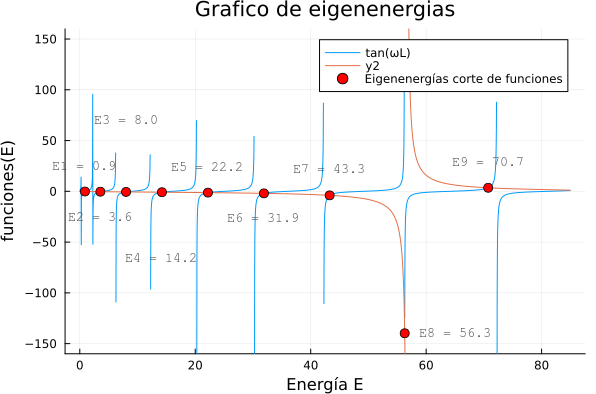
\includegraphics[width=0.8\linewidth]{figures/p2_energy_roots.png}
     \caption{Gráfica de la función tangente y la función que corresponden a las energías y choques con valores de energía de cada uno}
     \label{fig:placeholder}
 \end{figure}
 Para poder visualizar los engestados, podemos hacerlo con de manera más visual, poniendo las mismas funciones dentro del pozo. De esta manera vemos el fenómeno ondulatorio de nuestras 9 eigenenergias :
 
 \begin{figure}[H]
     \centering
     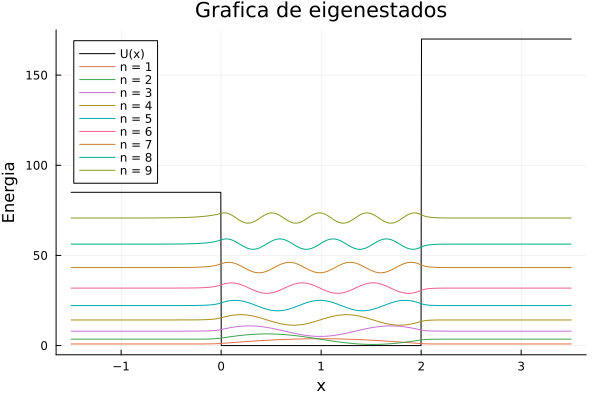
\includegraphics[width=0.8\linewidth]{figures/p2_eigenstates.png}
     \caption{Gráfica de eigenestados alrededor del pozo asimétrico, con respectivo número de eigenenergia}
     \label{fig:placeholder}
 \end{figure}
 Para este último es necesario recuperar primeramente el pulso gaussiano que se nos dio antes:
 \begin{equation}
\phi(x,0) = f(x; b, c) = A \exp\left[ -\frac{(x-c)^2}{b^2} \right] \exp\left( \mathrm{i}\frac{M v_0}{\hbar} x \right), \tag{5}
\end{equation}
Retomando entonces que el valor de A de la ecuación 1.36. Por lo que primero obtengamos los valores de $c_n$ para nuestros estados que lo haremos su proyección en nuestra base, para poder obtenerlo como en la ecuación 3.\\
De esta manera obtenemos los siguientes valores:
\begin{figure}[H]
    \centering
    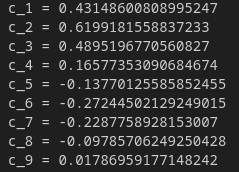
\includegraphics[width=0.3\linewidth]{figures/p2_expansion_coefficients.png}
    \caption{Valores de C encontrados de la base}
    \label{fig:placeholder}
\end{figure}
De esta manera podemos también elevar al cuadrado cada uno y encontrar la probabilidad de que al tener todos los estados nos dé 1, lo cual al hacerlo numéricamente nos da 0.9930, lo cual es muy cercano al 1, esto debido a que al no ser analítico tiene defectos.\\
Por lo que ahora construyamos la función de densidad de probabilidad, primero tomemos como antes g(x,t) que definimos de la siguiente manera:
\begin{equation}
    g(x,t) = \sum c_n \varphi_n e^{-iE_nt/\hbar}
\end{equation}
De esta manera podemos obtener los vectores que conforman nuestro vector, para poder obtener $g(x,t)^2$ debemos multiplicarlo por su conjugado por lo que al final modelaríamos algo como:
\begin{equation}
    P(x,t) = \sum_{n=1}^{N} \sum_{m=1}^{N} c_n c_m^* \varphi_n(x) \varphi_m(x) \exp \left[ -i \frac{(E_n - E_m)t}{\hbar} \right]
\end{equation}
Por lo que ahora podemos iterar esta misma fórmula con el fin de ir construyendo con respecto al tiempo nuestra función de probabilidad, con esto podemos construir un mapa de calor donde podamos ver como cambia $g(x,t)^2$ con el tiempo y como sus valores se ven más probables de estar en ciertos momentos.
\begin{figure}[H]
    \centering
    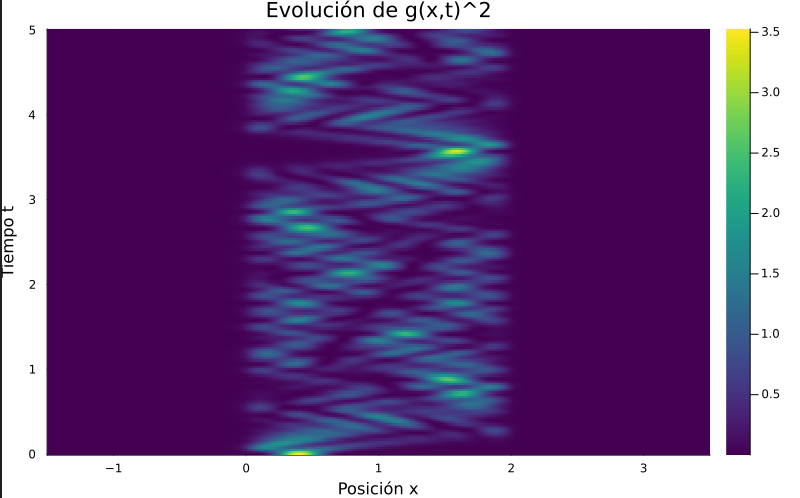
\includegraphics[width=0.5\linewidth]{figures/p2_gaussian_density.png}
    \caption{Mapa de calor sobre la evolución de la probabilidad en el espacio dentro del pozo también}
    \label{fig:placeholder}
\end{figure}
Por lo que ahora veamos el cálculo para el primer momento, recordemos el primer momento se puede ver también de la siguiente manera:  
\begin{equation*}
    <x>(t) = \int x P(x,t)dx
\end{equation*}
Por lo que podemos reutilizar el cálculo anterior de nuestra $g(x,t)^2$ para poder construir el primer momento y con su variación en el tiempo, resultando en la siguiente gráfica:
\begin{figure}[H]
    \centering
    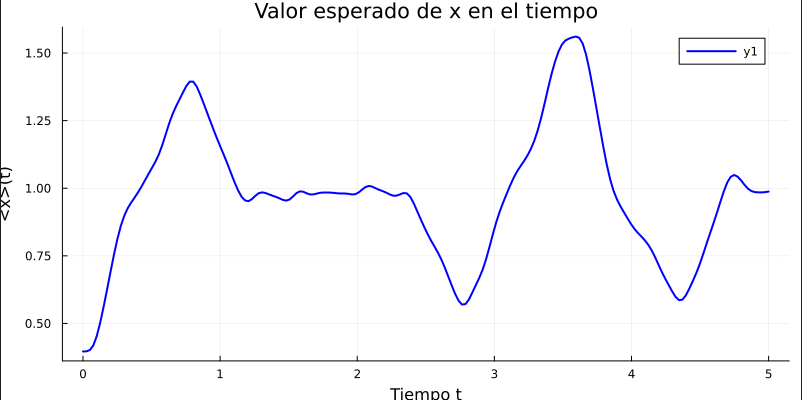
\includegraphics[width=0.5\linewidth]{figures/p2_gaussian_mean_position.png}
    \caption{Evolución temporal del valor esperado de x en 5 segundos}
    \label{fig:placeholder}
\end{figure}
Por lo que de esta manera obtenemos los momentos donde el valor esperado o el promedio de donde está la partícula contenida suele tener variaciones gracias a las energías que contiene, pero si podemos apreciar que se cumple que el valor inicial es el centro de nuestro pulso gaussiano en el tiempo 0.\\
\begin{figure}[H]
    \centering
    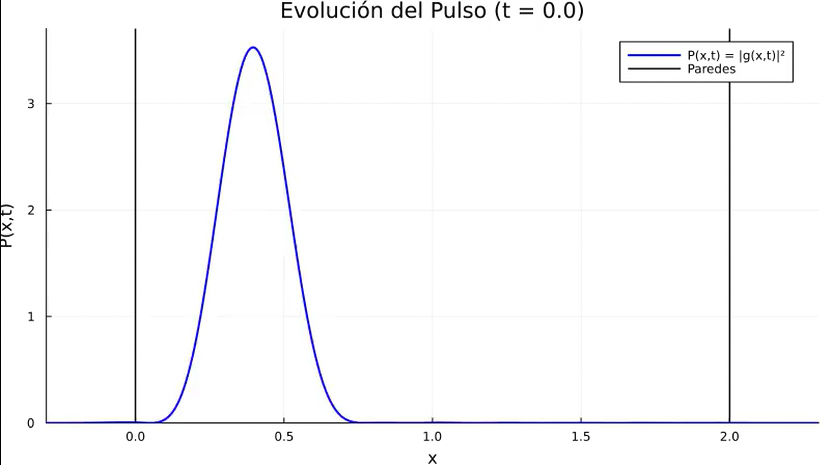
\includegraphics[width=0.5\linewidth]{figures/p2_video_frame.png}
    \caption{Captura del video del cambio de la probabilidad variando con respecto al tiempo}
    \label{fig:placeholder}
\end{figure}
Con esto finalmente podemos ver como la probabilidad de la partícula varía con el tiempo, siendo que inicialmente podemos ver nuestro pulso gaussiano. Es importante mencionar consideraciones físicas, como que nuestra gaussiana como se puede ver no tiene la altura suficiente para llegar a 4, esto se debe a la construcción de los 9 estados, es insuficiente a comparación de analíticamente donde si se pueda ver la representación completa.
\newpage

